\section{Delay Loop}

It is worth mentioning that the Delay Loop setup was performed always 
with 1.5~GHz beam with phase switches, i.e. the operational beam for 
factor 8 recombination. During initial years it was
started with 3~GHz beam because it offered better performance in terms
of stability, emittance and energy spread, therefore, it was easier to operate and setup.
It was thought that the setup for 1.5~GHz would be only a fast correction.
Unfortunately, it did not work this way and in all the cases the full commissioning
procedure had to be repeated with 1.5~GHz beam. On the other hand, in most cases the 3~GHz beam
was perfectly transported with the 1.5~GHz setup. It was understood
that the larger 1.5~GHz beam needed much more careful optics and orbit adjustments to fit within the \ac{DL} aperture. 
On the other hand the 3~GHz 
beam fitted well withing the 1.5~GHz print. 


\subsection{Injection}

During the initial setup the beam inevitably was entirely lost 
for some periods of time, therefore, the shortest possible beam pulse was used, 
usually 150~ns. The region of the straight section around the wigglers 
was particularly sensitive because particle showers were directed onto 
the hall entrance and were very likely to trigger radiation alarms.

The schema of the injection was described in Section~\ref{sec:DLinj}. 
Figure~\ref{fig:DLinj} shows the nominal beam trajectories with respect to the CT Line axis 
for beams injected to and bypassing the Delay Loop both 
with the RF Deflectors and with the magnetic correctors. 
The RF deflectors, correctors CT.DHD0495 and CT.DHD0505, BPI's CT.BPI0495 and CT.BPI0105 
were positioned 28.8~mm off the CT~Line axis to maximize the aperture for both, 
injected and ejected beams.
The reference trajectory, from which the element positionning was calculated, corresponded to
the beam guided with the RF deflectors, therefore their physical offset should be about 15~mm.
They could not be aligned perfectly and in reality they were offset by 16 and 17~mm.
%They were rigidly connected with the 5~m Y shape chamber connecting the CT line and the DL septa.
 
In order to facilitate operation the readings of 
CT.BPI0495 and CT.BPI0105 were visible with two configurations.
It was implemented by creating 2 controls devices for each of the monitors. 
The first one for the injected beam (\texttt{CT.STBPI0495} and \texttt{CD.STBPI0105}) and 
the second one for the bypassing beam (\texttt{CD.STBPI0495} and \texttt{CT.STBPI0105}).
Their delays and offsets in the read-out software were setup such that
the orbit display should read zero on all BPMs when operating the Delay Loop with the RF~deflectors, 
see Table~\ref{tab:DLinjBPMpars}.


\begin{table}
\centering
\begin{tabular}{@{}*{5}{c}@{}}
  Device name & pickup & \thead[c]{delay \\ {[ns]}} & \thead{physical \\ h. offset \\ {[mm]}} & \thead{software \\ h. offset \\ {[mm]}} \\
  \hline
  \texttt{CT.STBPI0495} & \texttt{CT.BPI0495} & 0   & 16 &  13.5 \\
  \texttt{CD.STBPI0105} & \texttt{CT.BPI0105} & 0   & 17 & -18.2 \\
  \texttt{CD.STBPI0495} & \texttt{CT.BPI0495} & 140 & 16 & -17.3 \\
  \texttt{CT.STBPI0105} & \texttt{CT.BPI0105} & 140 & 17 &  10.1 \\
\end{tabular}
\caption{Parameters of the beam position monitors at the \ac{DL} injection region.}
\label{tab:DLinjBPMpars}
\end{table}


\begin{figure}
\begin{center}
  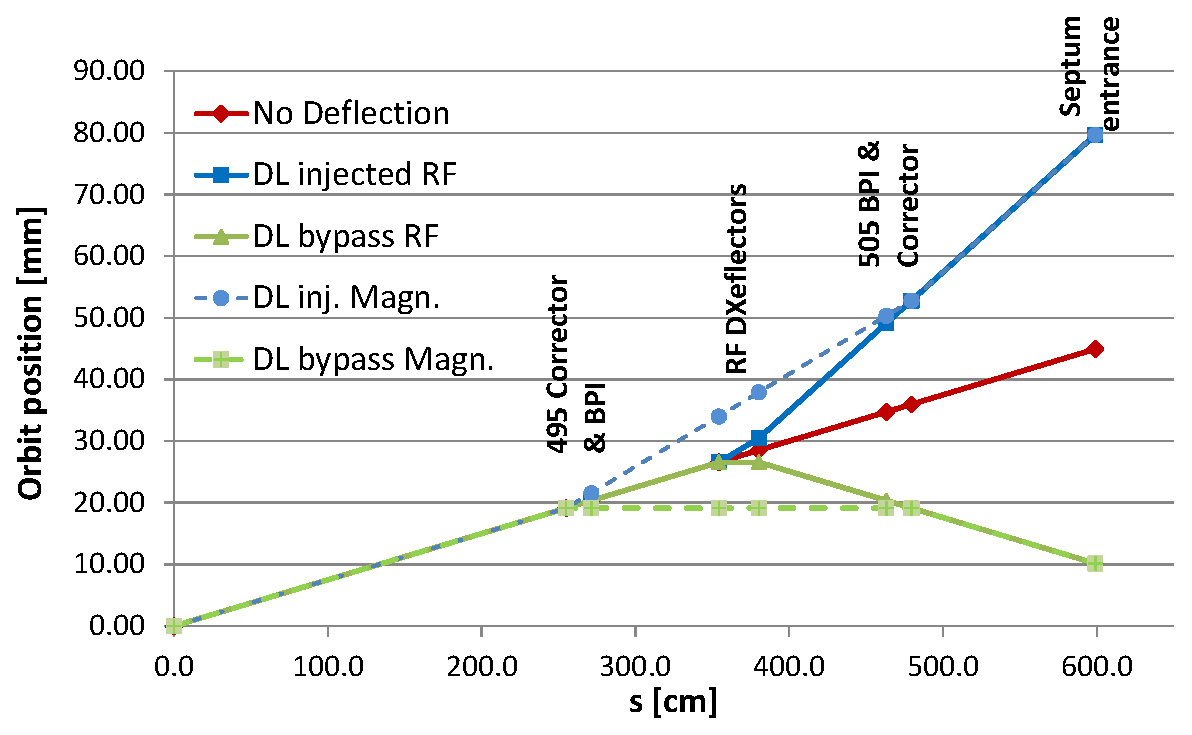
\includegraphics[width=0.7\linewidth]{DLinj.eps}
  \caption{Beam orbits through the \ac{DL} injection region from \texttt{CT.BHD0490} 
           to the septa entrance for different configurations. 
           Position values are with respect to the CT line axis.}
\label{fig:DLinj}
\end{center}
\end{figure}
\todo[inline]{values of the \ac{DL} inj orbit, plot from Excel}

First, magnetic injection was established. 
It was naturally much easier to setup and to operate comparing to the RF one. 
To be more efficient the \ac{DL} orbit and optics corrections were done with 
he magnetically injected beam.
Only when this beam had satisfactory performance the RF deflectors were started.

\begin{enumerate}
\item
The setup started with creation of the ``magnetic'' \ac{DL} injection orbit bump using 
\texttt{CT.BHD0490}, \texttt{CT.DHD0495}, \texttt{CT.DHD0505} and \texttt{CT.BHD0510} 
for the \ac{DL} bypassing beam. Its amplitude was adjusted to find the beam trajectory
in \texttt{CT.STBPI0495} and \texttt{CD.STBPI0105} at -1.2~mm and -30~mm, respectively.
A multi-knob application facilitated this task as it automatically dealt with the differences in 
the excitation constants of the involved magnets and any initial offsets defined by
prior orbit corrections. 
\item
Polarity of \texttt{CT.DHD0495} and \texttt{CT.DHD0505} orbit correctors was flipped 
in order to send the beam towards the septa. Its strength was adjusted 
with \texttt{CD.SHA0110-S} knob to find the beam centered at BPM CD.BPI0135. 
The current of the bends was adjusted to get best possible transmission
and orbit over maximum range. Eventually, manual or one-to-one orbit correction 
was performed to find the beam ejected from the loop and directed to the CTS dump. 
\item
In case a strong orbit correction was needed at the beginning or at the end of the loop then
it would mean that the injection bump and the septa were not well balanced.
The hight of the injection bump together with the powering of the septa were tuned 
to find an optimal angle for the injected and the ejected beam.
It was performed already when having the beam transported to the CTS dump
because this manipulation affected both the injection and the ejection.
The fact that all the septa magnets were powered in series made this coupling even stronger. 
Eventually, orbit before the \ac{DL} injection was adjusted when necessary. 
Both, beam directed to \ac{DL} and to \ac{TL1} were watched together to find an optimum condition.
\item
The orbit closure was performed with an automatic tool, see Section~\ref{sec:03_OrbitClosure}.
\item
After checking and correcting the optics, i.e. dispersion, $R_{56}$ and beta beating, 
the RF injection was established.
The orbits for the \ac{DL} bypassing beam as well as for the \ac{DL} were saved as references. 
Determining optimal amplitude and phase for the RF~deflectors was an iterative procedure
or it required finding relation between power and phase of MKL02 klystron, which was the deflectors RF source. 
In the latter case, for at least two different power levels 
the zero crossing phase was determined.
Keeping the beam at CTS or TL1 with the magnetic \ac{DL} bypass the RF~deflectors were powered. 
Klystron MKL02 phase was adjusted to bring the beam orbit on the reference 
what defined the first zero crossing phase. The second zero crossing naturally
should be 180 degrees apart. If not, calibration of the phase shifter had to be redone.
Linear fit to the obtained zero crossing phases versus klystron MKL02 power
gave the searched relation between the power and the phase.
If the iterative procedure was used then for each correction of the power level
%in the RF~deflectors 
the corresponding zero crossing had to be determined using the procedure above.
\item
In the last step correctors \texttt{CT.DHD0495} and \texttt{CT.DHD0505}
were switched off and phase of MKL02 shifted by 90 degrees.
MKL02 power was adjusted together with the phase (using the before found
relation) to get the orbit on the reference. Flipping the phase by 180 degrees
was making the beam injected into the \ac{DL}.
\item
Finally, the phase switches were enabled. 
As it was mentioned earlier in the description of the Injector setup, 
the switches could slightly modify the beam parameters.
Therefore the full setup procedure was eventaully repeated. 
Many iterations were eventally needed and achieving a satisfactory result 
was very difficult.
This was primarly because a correction of any parameter modified all the other parameters:
\textbeta-beating correction was modifing the orbit and dispersion,
dispertion correction was modifing the orbit and \textbeta-beating, etc. 
A global correction minimizing all the parameters all together would be a solution.
It was never tried at CTF3 for two reasons. 
First, a measurement of all the parameters together with the respective response matrices
was very time consuming and would need to be fully automatized.
Second, when it was coceived it was too late to implement 
\todo[inline]{finish the phrase}

%to fine tune the RF deflectors and the steering inside the loop.



\end{enumerate}


























